\documentclass{beamer}
\usepackage{amsmath}
\usepackage{bbm}
\usepackage{hyperref}
\usepackage{animate}
\usepackage{natbib}
\usepackage{algorithm}
\usepackage[noend]{algpseudocode}
\usepackage{placeins}
\usepackage{animate}
\usepackage{tikz}
\usetikzlibrary{positioning,shadows,arrows}
\usetheme{Berlin}
\usecolortheme{beaver}
\setbeamercolor{block title}{use=structure,fg=white,bg=darkred}
\setbeamercolor{block body}{use=structure,fg=black,bg=white!20!white}
\begin{document}
\title[Seminar, University of Basel]{Learning and distinguishing between active versions of prominent decision strategies}
\author[Schulz, Parpart, Meder, Love \& Speekenbrink]{Eric Schulz$^1$, Paula Parpart$^1$, \\Bj\"orn Meder$^2$, Bradley C. Love$^1$ \& Maarten Speekenbrink$^1$}
\institute{$^1$UCL London, Department of Experimental Psychology\\
$^2$MPI Berlin, Center for Adaptive Behavior and Cognition}
\date{\today}



\begin{frame}
\titlepage
\end{frame}

\begin{frame}
 \frametitle{If humans are active learners, then...}
\hfill \includegraphics[scale=0.05]{toolbox.jpg}\vspace{-2cm}
\begin{enumerate}
\item  ...how can they learn a heuristic that is made\\ 
up of building blocks on the fly when the\\
goal is to make good decisions?\bigskip\\\vspace{1cm}
 \hfill \includegraphics[scale=0.08]{tree.png}\vspace{-2cm}
\item ...how can we use that fact to test different\\ decision making strategies in an active learning\\
context?
\end{enumerate}
\end{frame}


\begin{frame}
 \frametitle{Overview}
 \begin{enumerate}
\item \textbf{Heuristics from Approximate Bayesian Computation}\\
\begin{center}
Collaborators:
\includegraphics[scale=0.07]{bjorn.jpg}Meder\hspace{0.5cm}
\includegraphics[scale=0.06]{maarten.jpg}Speekenbrink\hspace{0.5cm}
\end{center}
\begin{itemize}
\item How can a heuristic emerge from small building blocks?
\item Can a ABC method recover and/or outperform TTB?
\end{itemize}
\item \textbf{Distinguishing active versions of decision strategies}\\
\begin{center}
Collaborators:
\includegraphics[scale=0.013]{paula.jpg}Parpart\hspace{0.2cm}
\includegraphics[scale=0.2]{maarten2.jpg}Speekenbrink\hspace{0.2cm}
\includegraphics[scale=0.2]{brad.jpeg}Love
\end{center}
\begin{itemize}
\item How to distinguish between active versions of strategies?
\item How does the used strategy depend on the environment?
\end{itemize}
\end{enumerate}
\end{frame}

\begin{frame}
 \frametitle{PART 1: Can heuristics emerge/grow adaptively?}
\vspace{-1cm}
\begin{center}
\includegraphics[scale=0.1]{gerd.png}
\end{center}
\begin{itemize}
\vspace{-0.5cm}
\item Heuristics are made of smaller building blocks
\item Different combinations of blocks produce the heuritsic toolbox 
\item Definition of a heuristic:\medskip\\
\emph{``Ignores information to be faster and/or more accurate.''}\medskip\\
\emph{``Exhibits a starting rule, a search rule, and a stopping rule.''}
\end{itemize}
\end{frame}

\begin{frame}
 \frametitle{PART 1: Problem statement}
\begin{block}{Problem}
Given a number of binary cues $C_1, C_2, \dots, C_n$ --some of which might be invalid-- predict a binary outcome $y$ on every trial while at the same time learning a heuristic structure that consitsts of a starting, a search, and a stopping rule.
\end{block}
\textbf{Take-The-Best cannot deal with that, because...}
\begin{enumerate}
\item it is not clear how cue validities are learned
\item it is not clear how information is ignored
\item it cannot make decision and learn (evolve over time)
\item it is impossible to compute all valdities exactly on the fly
\end{enumerate}
\end{frame}

\begin{frame}
 \frametitle{PART 1: Approximate Bayesian Computation}
\textbf{How do you calculate a posterior when both analytical inference and sampling methods are intractable?}\medskip\\
Requirements: model $\mathcal{M}$, prior $\pi(\theta)$, data $\mathcal{D}=(\mathbf{X},\mathbf{y})$
\begin{enumerate}
\item Sample a proposal $\theta^*$ from your prior $\pi(\theta)$
\item Plug the proposal in your model $\mathcal{M}$ to get a model $\mathcal{M}^*$
\item Simulate $\mathbf{y}^*=\mathcal{M}^*(\mathbf{X})$
\item Calculate distance $\delta=\sum_i^n |y_i-y_i^*|$
\item If $\delta<\epsilon \rightarrow$ accept proposal \\
~~~~~else $\rightarrow$ reject proposal
\end{enumerate}
\end{frame}

\begin{frame}
 \frametitle{PART 1: Approximately Bayesian Computed TTB}
\textbf{How can TTB emerge from smaller buidling blocks?}\medskip\\
Requirements: urn containing the cues, for each cue: an urn containing the weights\\
urn has a pre-assigned number of $k$ balls for each class
\begin{enumerate}
\item Sample a cue $c^*$ from the cue urn without replacement
\item Sample a weight $w^*$ for $c^*$ from $c^*$'s weight urn
\item Encounter a situation $y_i$
\item If $y^*==y_i$ $\rightarrow$ put two more balls into $w^*$ and $c^*$\\
elseif $y^*==0$ $\rightarrow$ go back to 1\\
elseif $y^*\neq y_i$ $\rightarrow$ reject proposal, start again
\end{enumerate}
\end{frame}

\begin{frame}
 \frametitle{PART 1: Recovering TTB-The set up}
\begin{itemize}
\item 5 variables $x_1, x_2,x_3,x_4, x_5$, only the first three are valid
\item $p(x_k=W)=p(x_k=D)=p(x_k=L)=\frac{1}{3}$
\end{itemize}
\begin{figure}
\label{ttbtruth}
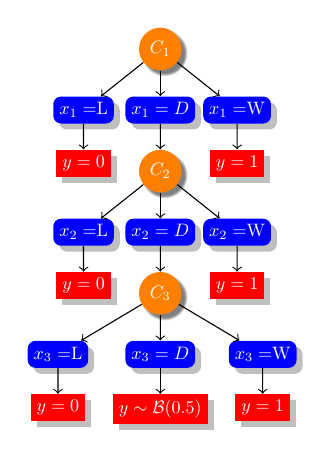
\begin{tikzpicture}[scale=0.65,transform shape,
    fact/.style={rectangle, draw=none, rounded corners=1mm, fill=blue, drop shadow,
        text centered, anchor=north, text=white},
    state/.style={circle, draw=none, fill=orange, circular drop shadow,
        text centered, anchor=north, text=white},
    leaf/.style={rectangle, draw=none, fill=red, drop shadow,
        text centered, anchor=north, text=white},
    level distance=0.5cm, growth parent anchor=south
]
\node (State00) [state] {$C_1$} [->]
child{
        node (Fact01) [fact] {$x_1=$L}
child{
                            node (State03) [leaf] {$y=0$}
                        }
        }
    child{
        node (Fact01) [fact] {$x_1=D$}
        child{
            node (State01) [state] {$C_2$}
           child{
        node (Fact04) [fact] {$x_2=$L}
child{
                            node (State05) [leaf] {$y=0$}
                        }
        } 
           child{
                node (Fact02) [fact] {$x_2=D$}
                child{ [sibling distance=2cm]
                    node (State02) [state] {$C_{3}$}
child{
        node (Fact31) [fact] {$x_3=$L}
child{
                            node (State33) [leaf] {$y=0$}
                        }
        }
                    child{[sibling distance=9cm]
                        node (Fact03) [fact] {$x_3=D$}
                        child{
                            node (leafguess) [leaf] {$y\sim \mathcal{B}(0.5)$}
                        }
                    }
child{
        node (Fact99) [fact] {$x_3=$W}
child{
                            node (State99) [leaf] {$y=1$}
                        }
        }
}}
child{
        node (Fact100) [fact] {$x_2=$W}
child{
                            node (State100) [leaf] {$y=1$}
                        }
        }
}}
child{
        node (Fact01) [fact] {$x_1=$W}
child{
                            node (State03) [leaf] {$y=1$}
                        }
        }

                    
;
        
\end{tikzpicture}
\end{figure}
\end{frame}

\begin{frame}
 \frametitle{PART 1: Recovering TTB: Results}
\begin{itemize}
\item Results
\begin{enumerate}
\item Can find the most important cues, even with a greedy strategy
\item Achieve an excellent misclassification rate
\item Can show mathematically that TTB-ABC corresponds to classic TTB if full set is sampled set 
\end{enumerate}
\item Current problems
\begin{enumerate}
\item How to avoid local optima (rescaling, jump starts, sampling)?
\item How to speed up computation (annealing, parallelization)?
\end{enumerate}
\end{itemize}
\end{frame}


\section{Introduction}
\begin{frame}
   \frametitle{Cue importance over time}
   \begin{figure}
\animategraphics[height=2.4in, autoplay]{10}{ttbabc/example}{1}{99}
     \end{figure}
\end{frame}


\begin{frame}
 \frametitle{PART 1: Empirical Test: City size data}
\hfill \includegraphics[scale=0.22]{germany.jpg}\vspace{-3cm}
\begin{itemize}
\item Most frequently used data sets within\\ the community
\item Predict which of two German cities has\\ 
the larger population size based on 9 cues
\item Take-The-Best is known to perform well
\item Cues have been pre-selected
\end{itemize}
\end{frame}

\begin{frame}
 \frametitle{PART 1: Empirical Test: Importance and direction}
\begin{center}
\includegraphics[scale=0.22]{ttbcity.pdf}
\end{center}
\end{frame}

\begin{frame}
 \frametitle{PART 1: Empirical Test: Model comparison}
\vspace{-0.2cm}
\begin{center}
\includegraphics[scale=0.37]{perfcitysize.pdf}
\end{center}
\end{frame}

\begin{frame}
 \frametitle{PART 1: Conclusion}
  \includegraphics[scale=0.12]{tools.jpeg}~TTB can emerge from simple building blocks over time\medskip\\
 \includegraphics[scale=0.07]{polya.png} Relies on simple sampling and approximate computation\medskip\\
\includegraphics[scale=0.05]{realtree.png} Can recover and perform as well as simple decision trees\bigskip\\
 \includegraphics[scale=0.12]{workinprogress.jpeg}~Speed, global optima, and experimental applications
\end{frame}


\begin{frame}
 \frametitle{PART 2: Can we distinguish different active algorithms?}
\vspace{-1cm}
\begin{center}
\includegraphics[scale=0.1]{gerdactive.png}
\end{center}
\begin{itemize}
\vspace{-0.5cm}
\item Agent has evolved to obey a certain decision algorithm
\item Agent learns with the goal to apply that algorithm 
\item Definition of active learning:\medskip\\
\emph{``Stepwise selection of observations in order to learn faster.''}\medskip\\
\emph{``Active learning leads to a banana shaped learning curve.''}
\end{itemize}
\end{frame}


\begin{frame}
 \frametitle{PART 2: Problem statement}
\begin{block}{Problem}
Given a number of binary cues $C_1, C_2, \dots, C_n$ --some of which might be invalid-- learn how to predict a binary outcome $y$ by selecting observations as wisely as possible.
\end{block}
\textbf{Current heuristics cannot deal with that, because...}
\begin{enumerate}
\item it is not clear how cue validities are learned
\item it is not clear how information is ignored
\item there are no active versions of them
\item active learning has never been utilized for model comparison
\end{enumerate}
\end{frame}

\begin{frame}
 \frametitle{PART 2: Model 1: Active TTB}
\begin{itemize}
\item \textbf{Imagine a scenario without noise:}\\
Every observation is deterministic and your only goal is, given your hypothesis space over all cue orders, $\mathcal{H}=\{\text{cue-order}_1, \text{cue-order}_2,\dots, \text{cue-order}_k\}$,
to select the observation $s^*=\text{argmax}\{|\mathcal{H}|-|\mathcal{H}|s|\}$ \\
\item Unfortunately, observations never come without noise
\item We have to find a probabilistic version of the same algorithm
\end{itemize}
\begin{center}
\includegraphics[scale=0.3]{hspace.png}
\end{center}
\end{frame}

\begin{frame}
 \frametitle{PART 2: Model 1: Active TTB algorithm}
\begin{itemize}
\item Put a pseudo-count $\pi$ over all possible cue orders
\item If a cue order makes a correct prediction, then $\pi++$
\item Calculate current entropy over all cue orders $S_0=\sum_i p_i \log p_i$
\item For every possible comparison $s$ calculate $p(y=w)$ and $p(y=L)$ by $\pi$-weighted sum over all cue orders
\item For every comparison $s$, calculate posterior expected entropy
$ \mathbb{E}[S|s]=S(y=W) \times p(y=W)+S(y=L) \times p(y=L)$
\item Choose $s^*=\text{argmax} \{S_0-\mathbb{E}[S|s]\}$, that is the observation with the highest expected information gain
\item Method works well a priori
\end{itemize}
\end{frame}

\begin{frame}
 \frametitle{PART 2: Model 2: Active Logistic Regression}
\begin{itemize}
\item Given a Bayesian variant of logistic regression:
\begin{center}
$f(x)=\frac{1}{1+\exp(-(\beta_0+\sum_k \beta_k x_k))}$
\end{center}
\item Calculate the current sum of coefficients' uncertainty
$S=\sum_k \mathbb{V}(\beta_k)$
\item For every comparison $s$, calculate $p(y=w|s)$ and $p(y=l|s)$
\item For every comparison and outcome calculate $S|s,y=w$ and $S|s,y=l$, that is the reduction of variance
\item For every comparison $s$, calculate posterior expected uncertainty
$ \mathbb{E}[S|s]=S(y=W) \times p(y=W)+S(y=L) \times p(y=L)$
\item Choose $s^*=\text{argmax} \{S_0-\mathbb{E}[S|s]\}$, that is the observation with the highest expected uncertainty reduction
\item Method works well a priori
\end{itemize}
\end{frame}

\begin{frame}
    \frametitle{Part 2: Alien Olympics:  Design}
\hfill \includegraphics[scale=0.14]{aliens.png}\vspace{-5cm}
\begin{enumerate}
\item Learn how well aliens perform in Olympics
\item Aliens vary on 4 different features:\\
Wings, Camouflage, Diamonds, and Antenn\ae
\item 30 learning trials: select 2 out of 4 aliens to\\
compete against each other (\$0.5 reward)
\item 10 test trials: select 1 out of 2 aliens for\\ your team (bonus dependent on team)
\item Environment set up with different levels of\\
compensatoriness
\end{enumerate}
\end{frame}

\begin{frame}
    \frametitle{Part 2: Alien Olympics:  Results in test set}
\hfill \includegraphics[scale=0.25]{comp.pdf}\vspace{-5cm}
\begin{enumerate}
\item Underlying envrionment obeys\\ logistic regression
\item Weights are generated by a\\ stick-breaking process\\
$\beta'_k \sim \text{Beta}(1,\theta)$\\
$\text{Define}~ \{\beta'_k\}^4_{k=1}\text{ as:}$\\
$\beta_k=\beta'_k\prod_{i=1}^{k-1}(1-\beta'_i) $
\item Allows to trade-off different\\ levels of compensatoriness
\end{enumerate}
\end{frame}

\begin{frame}
    \frametitle{Part 2: Alien Olympics:  Results of passive part}
 \includegraphics[scale=0.25]{score.pdf}\hspace{1cm}
 \includegraphics[scale=0.25]{percentage.pdf}
\begin{enumerate}
\item Non-compensatory conditions produce lower average score
\item Hard to distinguish between models based on test set alone
\end{enumerate}
\end{frame}


\begin{frame}
    \frametitle{Part 2: Alien Olympics:  Results of active part}
 \includegraphics[scale=0.3]{shortoverview.pdf}
 \includegraphics[scale=0.3]{results.pdf}
\vspace{-0.3cm}
\begin{enumerate}
\item Participants perform simple but sensible queries
\item Can distinguish between active models:\\
Only active TTB seems to match behavior well
\end{enumerate}
\end{frame}


\begin{frame}
 \frametitle{PART 2: Conclusion}
  \includegraphics[scale=0.12]{distinguish.jpeg}~Active learning can be used to distinguish different models \medskip\\
 \includegraphics[scale=0.6]{uncertain.png} It is possible to design active versions of classic models\medskip\\
\includegraphics[scale=0.07]{ttb.jpg}~~~In a first experiment, active TTB seems to do best\bigskip\\
 \includegraphics[scale=0.12]{workinprogress.jpeg}~Simpler follow-up, Exploitation scenarios, Non-parametrics
\end{frame}

\begin{frame}
 \frametitle{Overall conclusion}
\textbf{I hope to have convinced you that...}
\begin{enumerate}
\item ...active learning is an exciting tool to add to our methodological repertoire
\item ...it is both possible and fruitful to design active learning algorithms based on classic models
\item ...if we want to make claims about cognitive strategies, we also have to make claims about how those are acquired
\end{enumerate}
\textbf{Future steps could involve...}
\begin{enumerate}
\item ...coming up with more active learning models
\item ...designing additional active learning algorithms
\item ...modeling both exploration and exploitation scenarios
\end{enumerate}
\end{frame}

\begin{frame}
 \frametitle{Thanks you for your attention and to my collaborators}
\vspace{-0.3cm}
\begin{center}
\includegraphics[scale=0.1]{paula.png}\\
\includegraphics[scale=0.1]{bjorn.png}\\
\includegraphics[scale=0.1]{brad.png}\\
\includegraphics[scale=0.1]{maarten.png}
\end{center}
\end{frame}

\end{document}